\documentclass[11pt,a4paper]{article}

%==============================================================================%

\usepackage{a4wide}
\usepackage{amsmath,amssymb}
\usepackage[utf8]{inputenc}
\usepackage{float}
\usepackage{graphicx}
\usepackage{listings}
\usepackage{multicol}
\usepackage{tikz}

\usetikzlibrary{arrows}

%==============================================================================%

\newcommand{\assignmentnumber}{5}

\newcommand{\modulus}[1]{\left|#1\right|}
\newcommand{\conjugate}[1]{\bar{#1}}
\newcommand{\degree}{^{\circ}}
\newcommand{\limit}[2]{\lim_{#1 \rightarrow #2}}

\newcommand{\figref}[1]{fig. \ref{fig:#1}}
\newcommand{\eqnref}[1]{(\ref{eqn:#1})}

\DeclareMathOperator{\re}{Re}
\DeclareMathOperator{\im}{Im}

\renewcommand\thesection{\assignmentnumber.\arabic{section}}
\renewcommand\thesubsection{\alph{subsection})}

%==============================================================================%

\title{MatIntro Pointopgave \assignmentnumber}
\author
{
    Casper B. Hansen\\
    University of Copenhagen\\
    {\tt fvx507@alumni.ku.dk}
}
\date{\today}

%==============================================================================%

\begin{document}

% \maketitle


% 5.1
\section
{
    \mdseries
    Betragt funktionen $f(x,y) = \sqrt{4xy - 3y^2}$
}
I de følgende opgaver er følgende deklareret i Maple
\begin{lstlisting}
g := (x,y) -> 4xy - 3y^2
f := (x,y) -> sqrt(g(x,y))
\end{lstlisting}

\begin{multicols}{2}
    
    % 5.1 (a)
    \subsection
    {
        \mdseries
        Bestemt definitionsmængden $D_f$. Skitser (uden Maple) $D_f$ i et
        $xy$-diagram.
    }
    Under antagelsen om, at $f$ er en {\it reel} funktion er
    definitionsmængdien da $D_f = \{ (x,y) \in \mathbb{R}^2 | 4xy - 3y^2 \geq
    0 \}$.

    Løser vi for $y$ iht. ovenstående betingelse, får vi en ret linje, som
    viser $D_f$
    \begin{align}
        4xy - 3y^2 &= 0 \\
        3y^2 &= 4xy \\
        y^2 &= \frac{4}{3}xy \\
        y &= \frac{4}{3}x
    \end{align}

    \begin{figure}[H]
        \centering
        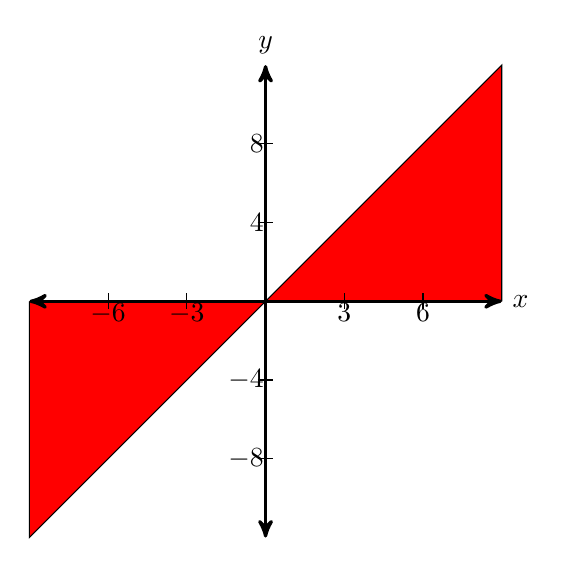
\begin{tikzpicture}[
            scale=1.0,
            axis/.style={very thick, <->, >=stealth'},
            vector/.style={thick, ->,color=red},
            important line/.style={thick},
            dashed line/.style={dashed, thin},
            pile/.style={thick, ->, >=stealth', shorten <=2pt, shorten
            >=2pt},
            every node/.style={color=black}
            ]

            \draw[fill=red] (0.0, 0.0) -- ( 3.0,  3.0) -- ( 3.0, 0.0);
            \draw[fill=red] (0.0, 0.0) -- (-3.0, -3.0) -- (-3.0, 0.0);

            % axis
            \draw[axis] (-3,0)  -- (3,0) node(xline)[right]{$x$};
            \draw[axis] (0,-3) -- (0,3) node(yline)[above]{$y$};

            \draw (-2.0, -0.1) -- (-2.0, 0.1) node[below]{$-6$};
            \draw (-1.0, -0.1) -- (-1.0, 0.1) node[below]{$-3$};
            \draw ( 1.0, -0.1) -- ( 1.0, 0.1) node[below]{$3$};
            \draw ( 2.0, -0.1) -- ( 2.0, 0.1) node[below]{$6$};

            \draw (-0.1, -2.0) -- (0.1, -2.0) node[left]{$-8$};
            \draw (-0.1, -1.0) -- (0.1, -1.0) node[left]{$-4$};
            \draw (-0.1,  1.0) -- (0.1,  1.0) node[left]{$4$};
            \draw (-0.1,  2.0) -- (0.1,  2.0) node[left]{$8$};

        \end{tikzpicture}
        \caption{Illustration af $D_f$ i $xy$-diagram.}
        \label{fig:5.1a}
    \end{figure}

    \vfill{\ }\columnbreak

    Bemærk at $x$-aksens intervaller er inddelt i multipla af $3$, og
    tilsvarende $y$-aksens intervaller er inddelt i multipla af $4$.

    % 5.1 (b)
    \subsection
    {
        \mdseries
        Lav (med Maple) et {\tt plot3d} af funktionen $4xy - 3y^2$, og
        sammensæt dette med et plot af $xy$-planen, således at uligheden
        $4xy - 3y^2 \geq 0$ illustreres.
    }
    I Maple skriver jeg
    \begin{lstlisting}
plot3d([f(x),0])
    \end{lstlisting}

    som giver figuren nedenfor
    \begin{figure}[H]
        \centering
        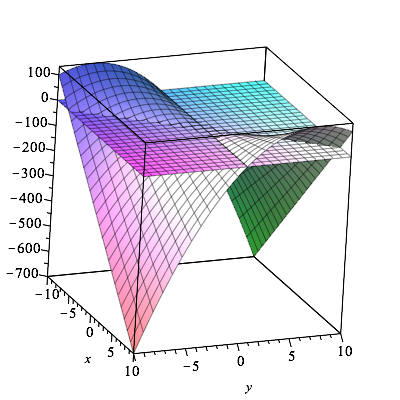
\includegraphics[scale=0.5]{figures/5-1b.png}
        \label{fig:5.1b}
        \caption{Grafen for $f$, samt $(x,y) = 0$.}
    \end{figure}

\end{multicols}

% 5.1 (c)
\newpage
\subsection
{
    \mdseries
    Bestem (uden Maple) $\limit{h}{0^+} \frac{f(h, rh)}{h}$ for alle $r \in
    [0,\frac{4}{3}]$.
}
Opstiller vi udtrykket, ser vi at vi kan faktorisere $h^2$ ud af kvadratroden,
og går derfor ud med nævneren. Vi har derfor, at
\begin{align}
    \limit{h}{0^+} \left( \frac{\sqrt{4 r h^2 - 3 r^2 h^2}}{h} \right)
     = \limit{h}{0^+} \left( \frac{h \sqrt{4 r - 3 r^2}}{h} \right)
     = \limit{h}{0^+} \left( \sqrt{4 r - 3 r^2} \right)
     = \sqrt{4 r - 3 r^2}
\end{align}

Bemærk, at $h$ er positiv som $h \rightarrow 0$ og derfor er grænseværdien også.

% 5.2
\section
{
    \mdseries
    Betragt funktionen $f(x) = x^4 + 7x^2 - 2$.
}

% 5.2 (a)
\subsection
{
    \mdseries
    Bestem alle Taylorpolynomierne omkring $x = 1$ for funktionen (uden
    Maple).
}
\begin{multicols}{2}
    Først differenerer vi $f$ fire gange, da $f$ er et fjerdegradspolynomium.
    Og beregner tilhørende koefficienter.
    \begin{align}
        f     &= x^4 + 7x^2 - 2 \qquad f(1) = 6 \\
        f'    &= 4x^3 + 14x \qquad f'(1) = 18 \\
        f''   &= 12x^2 + 14 \qquad f''(1) = 26 \\
        f'''  &= 24x \qquad f'''(1) = 24 \\
        f'''' &= 24 \qquad f''''(1) = 24
    \end{align}

    Vi kan da beregne $T_0 f(x)$

    \begin{align}
        T_0 f(x) = f^{(0)}(1) (x - 1)^0 = 6
    \end{align}

    Og følgende $T_k f(x)$, for $k \in [1,4]$

    \begin{align}
        T_1 f(x) &= T_0 f(x) + \frac{f^{(1)}(1)}{1} (x - 1)^1 \\
                 &= 6 + 18(x - 1) = 18x - 12
    \end{align}

    \begin{align}
        T_2 f(x) &= T_1 f(x) + \frac{f^{(2)}(1)}{2} (x - 1)^2 \\
                 &= 18x - 12 + 13(x^2 + 1 - 2x) \\
                 &= 13x^2 - 8x + 1
    \end{align}

    \vfill{\ }\columnbreak

    \begin{align}
        T_3 f(x) &= T_2 f(x) + \frac{f^{(3)}(1)}{6} (x - 1)^3 \\
                 &= 13x^2 - 8x + 1 + 4(x - 1)^3 \\
                 &= 4x^3 + x^2 + 4x - 3
    \end{align}

    \begin{align}
        T_4 f(x) &= T_3 f(x) + \frac{f^{(4)}(1)}{24} (x - 1)^4 \\
                 &= 4x^3 + x^2 + 4x - 3 + (x - 1)^4 \\
                 &= x^4 + 7x^2 - 2
    \end{align}

    Bemærk, at $f(x) = T_4 f(x)$.

    \begin{figure}[H]
        \centering
        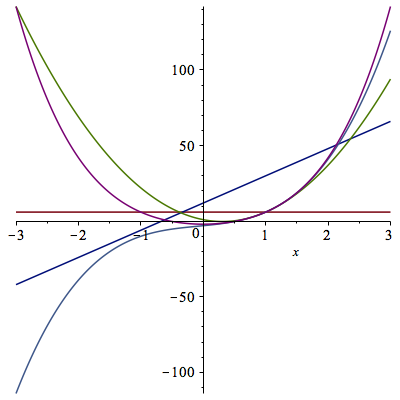
\includegraphics[scale=0.4]{figures/5-2b.png}
        \label{fig:5.2b}
        \caption{Graferne for hhv. $T_1 f$ (rød), $T_2 f$ (blå) og $T_3 f$
        (grøn), samt $f$ (gul).}
    \end{figure}

    \vfill{\ }

\end{multicols}

% 5.2 (b)
\subsection
{
    \mdseries
    Indtegn (med Maple) resultatet fra (a) i et plot, som viser grafen for $f$
    samt de tre Taylorpolynomier $T_1 f$, $T_2 f$ og $T_3 f$. Vælg f. eks.
    $x$-intervallet $[-3,3]$.
}
Se figur 3 i opgave (a).

% 5.3i
\section
{
    \mdseries
    Betragt den naturlige logaritmefunktion $f(x) = \ln x$, og lad $T_n \ln$
    være Taylorpolynomiet af grad $n$ omkring $x = 1$. Benyt formlen (side
    586) for den $n$-te afledte af $\ln$, $f^{(n)}(x) = (-1)^{n - 1}
    (n - 1)!x^{-n}$.
}

% 5.3i (a)
\subsection
{
    \mdseries
    Plot (med Maple) graferne for $\ln$, $T_9 \ln$ og $T_{49} \ln$ i et
    fælles plot.
}

\begin{multicols}{2}

    Først beregner vi de afledte
    \begin{align}
        f^{(9)} = (-1)^{9-1} (9 - 1)! x^{-9}
                = \frac{8!}{x^9} \\
        f^{(49)} = (-1)^{49-1} (49 - 1)! x^{-49}
                 = \frac{48!}{x^{49}}
    \end{align}
    og tilhørende funktionsværdier omkring $x = 1$
    \begin{align}
        f^{(9)} (1) &= 8! \\
        f^{(49)} (1) &= 48!
    \end{align}

    I Maple skriver jeg
    \begin{lstlisting}
f := ln(x)
T9 := mtaylor(f(x), x=1, 9)
T49 := mtaylor(f(x), x=1, 49)

plot([T9,T49], x=-2..4, y=-10..2)
    \end{lstlisting}
    hvilket giver grafen i figur 4, vist til højre.

    \vfill{\ }\columnbreak

    \begin{figure}[H]
        \centering
        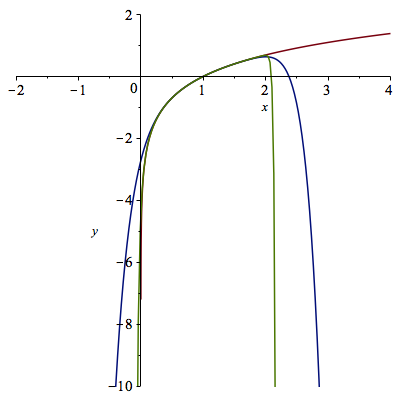
\includegraphics[scale=0.4]{figures/5-3a.png}
        \label{fig:5.3a}
        \caption{Graferne for $\ln x$ (rød), $T_9$ (blå) og $T_49$ (grøn).}
    \end{figure}

\end{multicols}

% 5.3i (b)
\subsection
{
    \mdseries
    Argumentér, ud fra Taylors formel med restled, for at $\modulus{R_n
    \ln x} = \modulus{\ln x - T_n \ln x} \leq \frac{1}{n+1}(x-1)^{n+1}$ for
    $x > 1$. Udregn (med Maple), for $x = 2$, $x = 1.9$ og $x = 2.1$, værdien
    af $T_{49} \ln x$ og sammenlign med $\ln x$ (også udregnet i Maple).
    Check uligheden ovenfor. Forklar forskellen mellem tilfældene $x < 2$ og
    $x > 2$.
}
Hvis vi indsætter i Lagranges restledsformel og erstatter $f^{(n+1)}$ med den
givne formel, får vi
\begin{align}
    \modulus{R_n \ln x} &= \modulus{ \frac{f^{(n+1)} (c)}{(n + 1)!} (x - 1)^{n+1} }
    \\\implies
    \modulus{R_n \ln x}
    &= \modulus{ (-1)^n \frac{n! c^{-(n + 1)}}{(n + 1)!} (x - 1)^{n+1} }
    = \modulus{ \frac{1}{c^{n + 1}(n + 1)} (x - 1)^{n+1} }
\end{align}

Idet $1 < c < x$ jvf. definitionen af Lagranges restledsformel har vi, at
$c^{n+1} (n + 1) > (n + 1)$ og derfor holder uligheden, da nævneren i
restledet, som beregnet, da altid vil være større.

\begin{multicols}{2}
    For $T_{49} \ln x$ skriver jeg i Maple
    \begin{lstlisting}
T := mtaylor(f(x), x=1, 49)
evalf(subs(x=2, T))
evalf(subs(x=1.9, T))
evalf(subs(x=2.1, T))
    \end{lstlisting}
    og ligeledes for $\ln x$
    \begin{lstlisting}
evalf(ln(2))
evalf(ln(1.9))
evalf(ln(2.1))
    \end{lstlisting}
    
    hvilket giver mig
    \begin{align}
        T_{49} \ln x =  0.68283900 \text{, for } x &= 2 \\
        T_{49} \ln x =  0.64179181 \text{, for } x &= 1.9 \\
        T_{49} \ln x = -0.30627131 \text{, for } x &= 2.1
    \end{align}
    og tilsvarende
    \begin{align}
        \ln 2.0 = 0.69314718 \\
        \ln 1.9 = 0.64185389 \\
        \ln 2.1 = 0.74193734
    \end{align}
    
    \vfill{\ }\columnbreak

    I modsætning til $\ln x$, som er voksende i hele $\mathbb{R}$, har vores
    Taylorpolynomium approksimering vendetangent i $x = 2$, altså $x = 2$ er
    en løsning til $T_{49}' = 0$, og er aftagende i $[2,\infty)$. Dette
    fremgår også tydeligt af figur 4. Denne egenskab ved $T_{49}$ afviger
    stærkt fra $\ln x$.

\end{multicols}

\end{document}
